% Macro definitions needed for this chapter
\newcommand{\promptExampleSize}{\small}
\newcommand{\promptstyle}[1]{``{\promptExampleSize \texttt{#1}}''}

\section{Dataset}
\label{magick_sec:method}

The MAGICK\ dataset is a collection of 150,000 objects extracted from generated images. Each object consists of 1) an image of the object with pure foreground colors (i.e. no background color is mixed into edge and transparent pixels), 2) the alpha matte of the object, and 3) the caption used to generate the object. The wide variety of objects is not restricted to any small set of given object classes. Many of the objects exhibit details that require a detailed matted such as hair, fur, thin parts, or transparencies.

\cref{magick_fig:datasetExpose} shows 100 examples from our dataset. As can be seen, the object types vary widely and the alpha mattes contain accurate details.

Generating a dataset like MAGICK\ is non-trivial. No existing generation model can produce accurate images with alphas. Datasets with accurate alpha are limited, making it difficult to train such a method. While existing segmentation or matting methods could be applied to generated images to extract objects, such methods are imperfect and would not yield results suitable for representing ground-truth for training. To accomplish this, we needed to use a combination of generation and alpha extraction methods.

\subsection{Dataset Creation}

\begin{figure}
    \centering
    \includegraphics[width=1\linewidth]{src/3_MAGICK/figs/PipelineOverview.png}
    \caption[Overview of the MAGICK dataset generation pipeline]{A general overview of our pipeline for image generation.}
    \label{magick_fig:pipelineOverview}
\end{figure}

To create MAGICK, we generate objects on a green screen (or other constant colored screen) so that ground-truth quality results can be extracted. While chroma keying from green screen footage is common, doing this at scale with generation faces several challenges. In addition to requiring a large set of prompts, we must have a way to select the background color automatically, to generate a object on a colored background that is suitable for chroma keying, and to extract the alpha automatically. We propose a method to overcome these challenges.

The overview is shown in Fig.~\ref{magick_fig:pipelineOverview}. First, a prompt is chosen. Then, a suitable color for the background is chosen by generating an image from that prompt and analysing its distribution of hues. Next, a \emph{keyable} image, or image that is suitable for chroma keying, is created by chaining together two diffusion models, DeepFloyd~\cite{deepfloyd} and SDEdit~\cite{sdedit} with SDXL~\cite{podell2023sdxl}. Finally, multiple alpha extraction methods are run and the best matte is chosen.

\subsubsection{Selecting Prompts}
\label{magick_sub:selecting_prompts}

The first step in generating our large synthetic image dataset is to come up with a list of prompts. As we will be engineering the prompts with additional descriptions in later steps, we will refer to the part of the prompt that describes the object as the ``subject''. The subject must highlight and meaningfully describe a single subject in each image without mentioning other objects or background details so that it can be easily isolated from the background.

We obtain the subjects in our dataset from three sources:
1) Outputs from LLMs such as GPT-4 and ChatGPT,
2) Procedurally generated subjects for humans, and
3) Captions from an existing image-caption datasets

\paragraph{LLM-Generated Prompts}

Recent large language models (LLMs) have proven capable of generating text given a prompt. We leverage this by using ChatGPT and GPT4 to create subject prompts. We instruct the LLMs to write a descriptive caption of an object in an image without describing the background or other objects. We provide LLMs with a list of object categories, both general objects and objects with details that require complex mattes like hair, fur, or transparent parts, but also allow the LLMs to extrapolate their own categories for additional variety.

Examples of captions created using LLMs include  \promptstyle{A detailed macro shot of a butterfly wing} and \promptstyle{A piece of amber glass reflecting sunlight.}  Additional examples and the LLM prompt we use can be found in the appendix.

\paragraph{Procedurally Generated Prompts}
Because humans are an important part of our dataset, we created a template mechanism for procedurally constructing descriptions of humans. We focused on diversity, attempting to capture many different professions, ethnicities, clothing, accessories, genders and hairstyles.
Some example subjects are \promptstyle{lawyer woman diamond earrings}, \promptstyle{person wearing gown}, and \promptstyle{hispanic barista man with black flowing hair}. More examples can be found in the appendix.

\paragraph{Image Captions}
While many image captioning datasets exist~\cite{chen2015microsoft,young2014from,sharma2018conceptual}, their captions typically describe the scene and potentially multiple objects, such as the caption \promptstyle{A large bus sitting next to a very tall building} from~\cite{chen2015microsoft}.  Such captions are not suitable for our needs as identifying the subject is difficult.

We instead extract subjects from a proprietary image-caption dataset. In addition to the full scenes present in prior datasets, this dataset also includes images of isolated objects. The captions of such objects often contain identifying words such as ``clipping path'', ``greenscreen'', or ``on a white background''. We search for such tags and remove them from the caption. This yields descriptive subjects such as `\promptstyle{Close-up of a new basketball ball} and  \promptstyle{White and brown chicken wings}. More examples can be found in the appendix.

\subsubsection{Finding the Least Common Hue}
\label{magick_sub:least_common_hue}
For our approach, we must generate images with solid colored backgrounds for chroma keying. To do this, we must choose a background color that does not conflict with the subject, as that would render any chroma keying algorithm useless. It is well-known that wearing a green shirt against a green screen will causes your torso disappear in the output.

To find an appropriate background color for a given subject, we follow the procedure depicted in \cref{magick_fig:leastCommonHueHistogram}. First, for a given subject, we generate an image using SDXL with the subject (unmodified) as the prompt. While this generated image will not be on a solid colored background as we need for alpha extraction, it will typically show the color distribution for that given subject. We create a histogram of the hues of the pixels in the generated image weighted by saturation, then smooth the hue histogram with a Gaussian kernel with
$\sigma=10^\circ$.  We quantize the histogram into regions representing named colors (e.g. green, blue, etc) and return the color name as a string. This string representing the hue will be used to generate the image in the next step.

We found that ``green'' and ``blue'' are by far the most common background colors in our dataset, totaling over 90\%
of images. This matches practical experience where objects to be chroma keyed are almost always shot against a green or blue screen. This is also partially due to the wide band of hues that these colors cover.

\begin{figure}
    \centering
    \includegraphics[width=1\linewidth]{src/3_MAGICK/figs/LeastCommonHueHistogram.png}
    \caption[Finding the least common hue for background selection]{Finding the least common hue of a given subject. In this example, ``green'' is least common.}
    \label{magick_fig:leastCommonHueHistogram}
\end{figure}

\subsubsection{Generating \emph{Keyable} Images}

Give a subject and a background color, we can now generate an image from which we will extract the alpha. For this to work, the image must be \emph{keyable}. For an image to be \emph{keyable}, it 1) must have a constant, bright, saturated background color, 2) must not have any objects or gradients in the background, 3) must have fine details like hair, fur, and transparencies in the object when appropriate, and 4) must not have color spill, or background colors tinting the foreground.

Unfortunately, all the publicly available methods we tested were incapable of consistently creating \emph{keyable} images. As shown in Fig.~\ref{magick_fig:greenscreenComparison}, SDXL, Midjourney, Dalle, and Stable Diffusion often produce backgrounds that are not suitable for extraction (being too dark, desaturated, or having gradients or objects) or have color spill. DeepFloyd is quite good at generating vibrant clean backgrounds and foreground with no color spill but fails to produce soft edges (see the lion's mane in~\cref{magick_fig:greenscreenComparison}).

Because of these shortcomings, we propose combining multiple generation methods (namely DeepFloyd and SDEdit) with the goal of overcoming these weaknesses through the combination. Our process is described below.

\begin{figure}
    \centering
    \includegraphics[width=1\linewidth]{src/3_MAGICK/figs/priorcomparison.png}
    \caption[Comparison of diffusion models for green screen generation]{We compare results from multiple diffusion models. Each algorithm produces images that are not \emph{keyable}, either the foreground has no fine detail or is tinted green or the background is not suitable for chroma keying. Please zoom in for details.
    }
    \label{magick_fig:greenscreenComparison}
\end{figure}

\paragraph{Prompt engineering}
We first augment the subject to indicate the background color. For example, if the background color were ``green'', we augment the subject with the phrase \promptstyle{isolated on a solid green background}.

\paragraph{Image generation}
To create a \emph{keyable} image, we use both the text-to-image generation method DeepFloyd followed by the image-to-image generation methods SDEdit. This process is illustrated in \cref{magick_fig:imgToImgPipeline}.

First, we use our prompt with DeepFloyd to generate an initial image. We found that DeepFloyd could consistently produce suitable backgrounds but the foregrounds were lacking detail in the alpha. However, the backgrounds are often not as bright and saturated needed for SDEdit. To address this, we perform an initial extraction of the object and composite it onto a brighter, more saturated background with the approximately same hue. We use Photoshop's Subject Selection feature, a method that uses deep-learning-based segmentation and matting to compute masks for primary objects in an image and can be run in batch mode.  This method does not perfectly extract the object and may leave green pixels in regions like hair, but these typically do not cause a problem as the object is immediately composited onto a similar colored background.

We then use SDEdit \cite{sdedit}, the image-to-image version of SDXL implemented by Huggingface \cite{huggingface_img2img}, to regenerate the final image.  In this step, we need to guarantee that the object has fine details, that it has no color spill, and that the background is solid, bright, and saturated enough for chroma keying. To produce fine details, we set SDEdit's strength parameter to .95. This parameter, ranging from 0 to 1, determines how closely the generation follows the input image by modulating the amount of noise added to the image. This allows enough freedom for SDEdit to generate a new version of the same object with better details, not only at the edges but often in the interior of the object as well. To prevent color spill, we add the background color as a negative prompt. This suppresses that color in the foreground object, but because the background is so bright and saturated from the previous step it fails to suppress the color in the background.

\cref{magick_fig:beforeAfterImg2Img} shows the impact of this process. The images in the column ``Before Img2Img'' are the outputs from DeepFloyd after being matted by Photoshop Subject Selection and composited onto a solid background, and the ``AfterImg2Img'' column are the outputs of SDEdit. Note the fidelity of the image increases and any color spill corrected due to the negative prompt. (e.g. the submarine's green tint or the girl's green dress). Also note the mistakes made by Photoshop Subject Selection are corrected as well - the dandelions look poorly extracted before SDEdit but look natural after.

Despite these efforts to make the images as \emph{keyable} as possible, our process is imperfect, sometimes yielding results with gradients in the background color or tinting of the foreground object. To deal with this, we require a robust alpha computation method.

\begin{figure}
    \centering
    \includegraphics[width=1\linewidth]{src/3_MAGICK/figs/img2img_pipeline.pdf}
    \caption[Image generation pipeline using DeepFloyd and SDXL]{We generate the RGB images in our dataset using a combination of both DeepFloyd, Photoshop's Subject Selection feature, and Stable Diffusion XL. The resulting images have near-perfect, high saturation backgrounds that are ideal for chroma keying. Please zoom in for details.}
    \label{magick_fig:imgToImgPipeline}
\end{figure}

\begin{figure}
    \centering
    \includegraphics[width=1\linewidth]{src/3_MAGICK/figs/BeforeAfterImg2ImgFlat3.pdf}
    \caption[Effect of SDEdit on DeepFloyd-generated images]{Examples of image before and after applying image-to-image SDEdit. The before images are outputs of DeepFloyd after being extracted by Photoshop Subject Selection and composited onto a new background. Please zoom in for details.}
    \label{magick_fig:beforeAfterImg2Img}
\end{figure}

\subsubsection{Alpha extraction}

Once we have a \emph{keyable} image, we must extract the alpha from the image. Unfortunately, this is also a difficult process. Chroma keying is an underconstrained problem. Even with a solid background color, chroma keying methods can fail to correct compute the alpha, and in practice users must manually change parameters or correct the mattes for a high quality result. This time-consuming process does not scale to large datasets.

To address this, we generate three alpha mattes and choose between them. These three methods operate differently and in difficult cases one algorithm may compute accurate results when the other cannot.
The algorithms we use are:
\\
1. \textit{A pixel-based chroma key method}. We modified a traditional color difference chroma key algorithm~\cite{wright2010taylor} that takes a single rgb color representing the background as input to instead take a background rgb color per pixel. We conservatively delete the foreground object and inpaint the background using \cite{Telea2004}  to provide the background color at each pixel. This allows us to better handle subtle gradients in the background color. Note that this also performs color decontamination in the same step.
\\
2. \textit{A deep-learning based chromakey model} that was trained on an internal dataset and takes in an input RGB image and a background RGB image and returns the alpha and foreground color.
\\
3. \textit{Photoshop's Subject Selection} which uses proprietary segmentation and matting algorithms to select the primary object in an image. It works well on images with simple backgrounds and is robust to color spill.

\cref{magick_fig:alpha_compare} compares the three methods on three examples, highlighting cases where the methods have inconsistent results. In such cases, one of the methods is able to compute an accurate alpha.

Recalling the image matting equation:
\begin{equation}\label{magick_eq:compositing_equation}
  I = \alpha F + (1-\alpha) B,
\end{equation}
we require not just the alpha but also $F$, the pure foreground color of the pixel with any background color $B$ removed. Each of our three alpha extraction methods generate a predicted $F$. However, the method that predicts the best alpha does not necessarily also produce the best $F$. Experimentally, we chose the best seven combinations as possible choices for the final alpha and $F$.


\begin{figure}
    \centering
    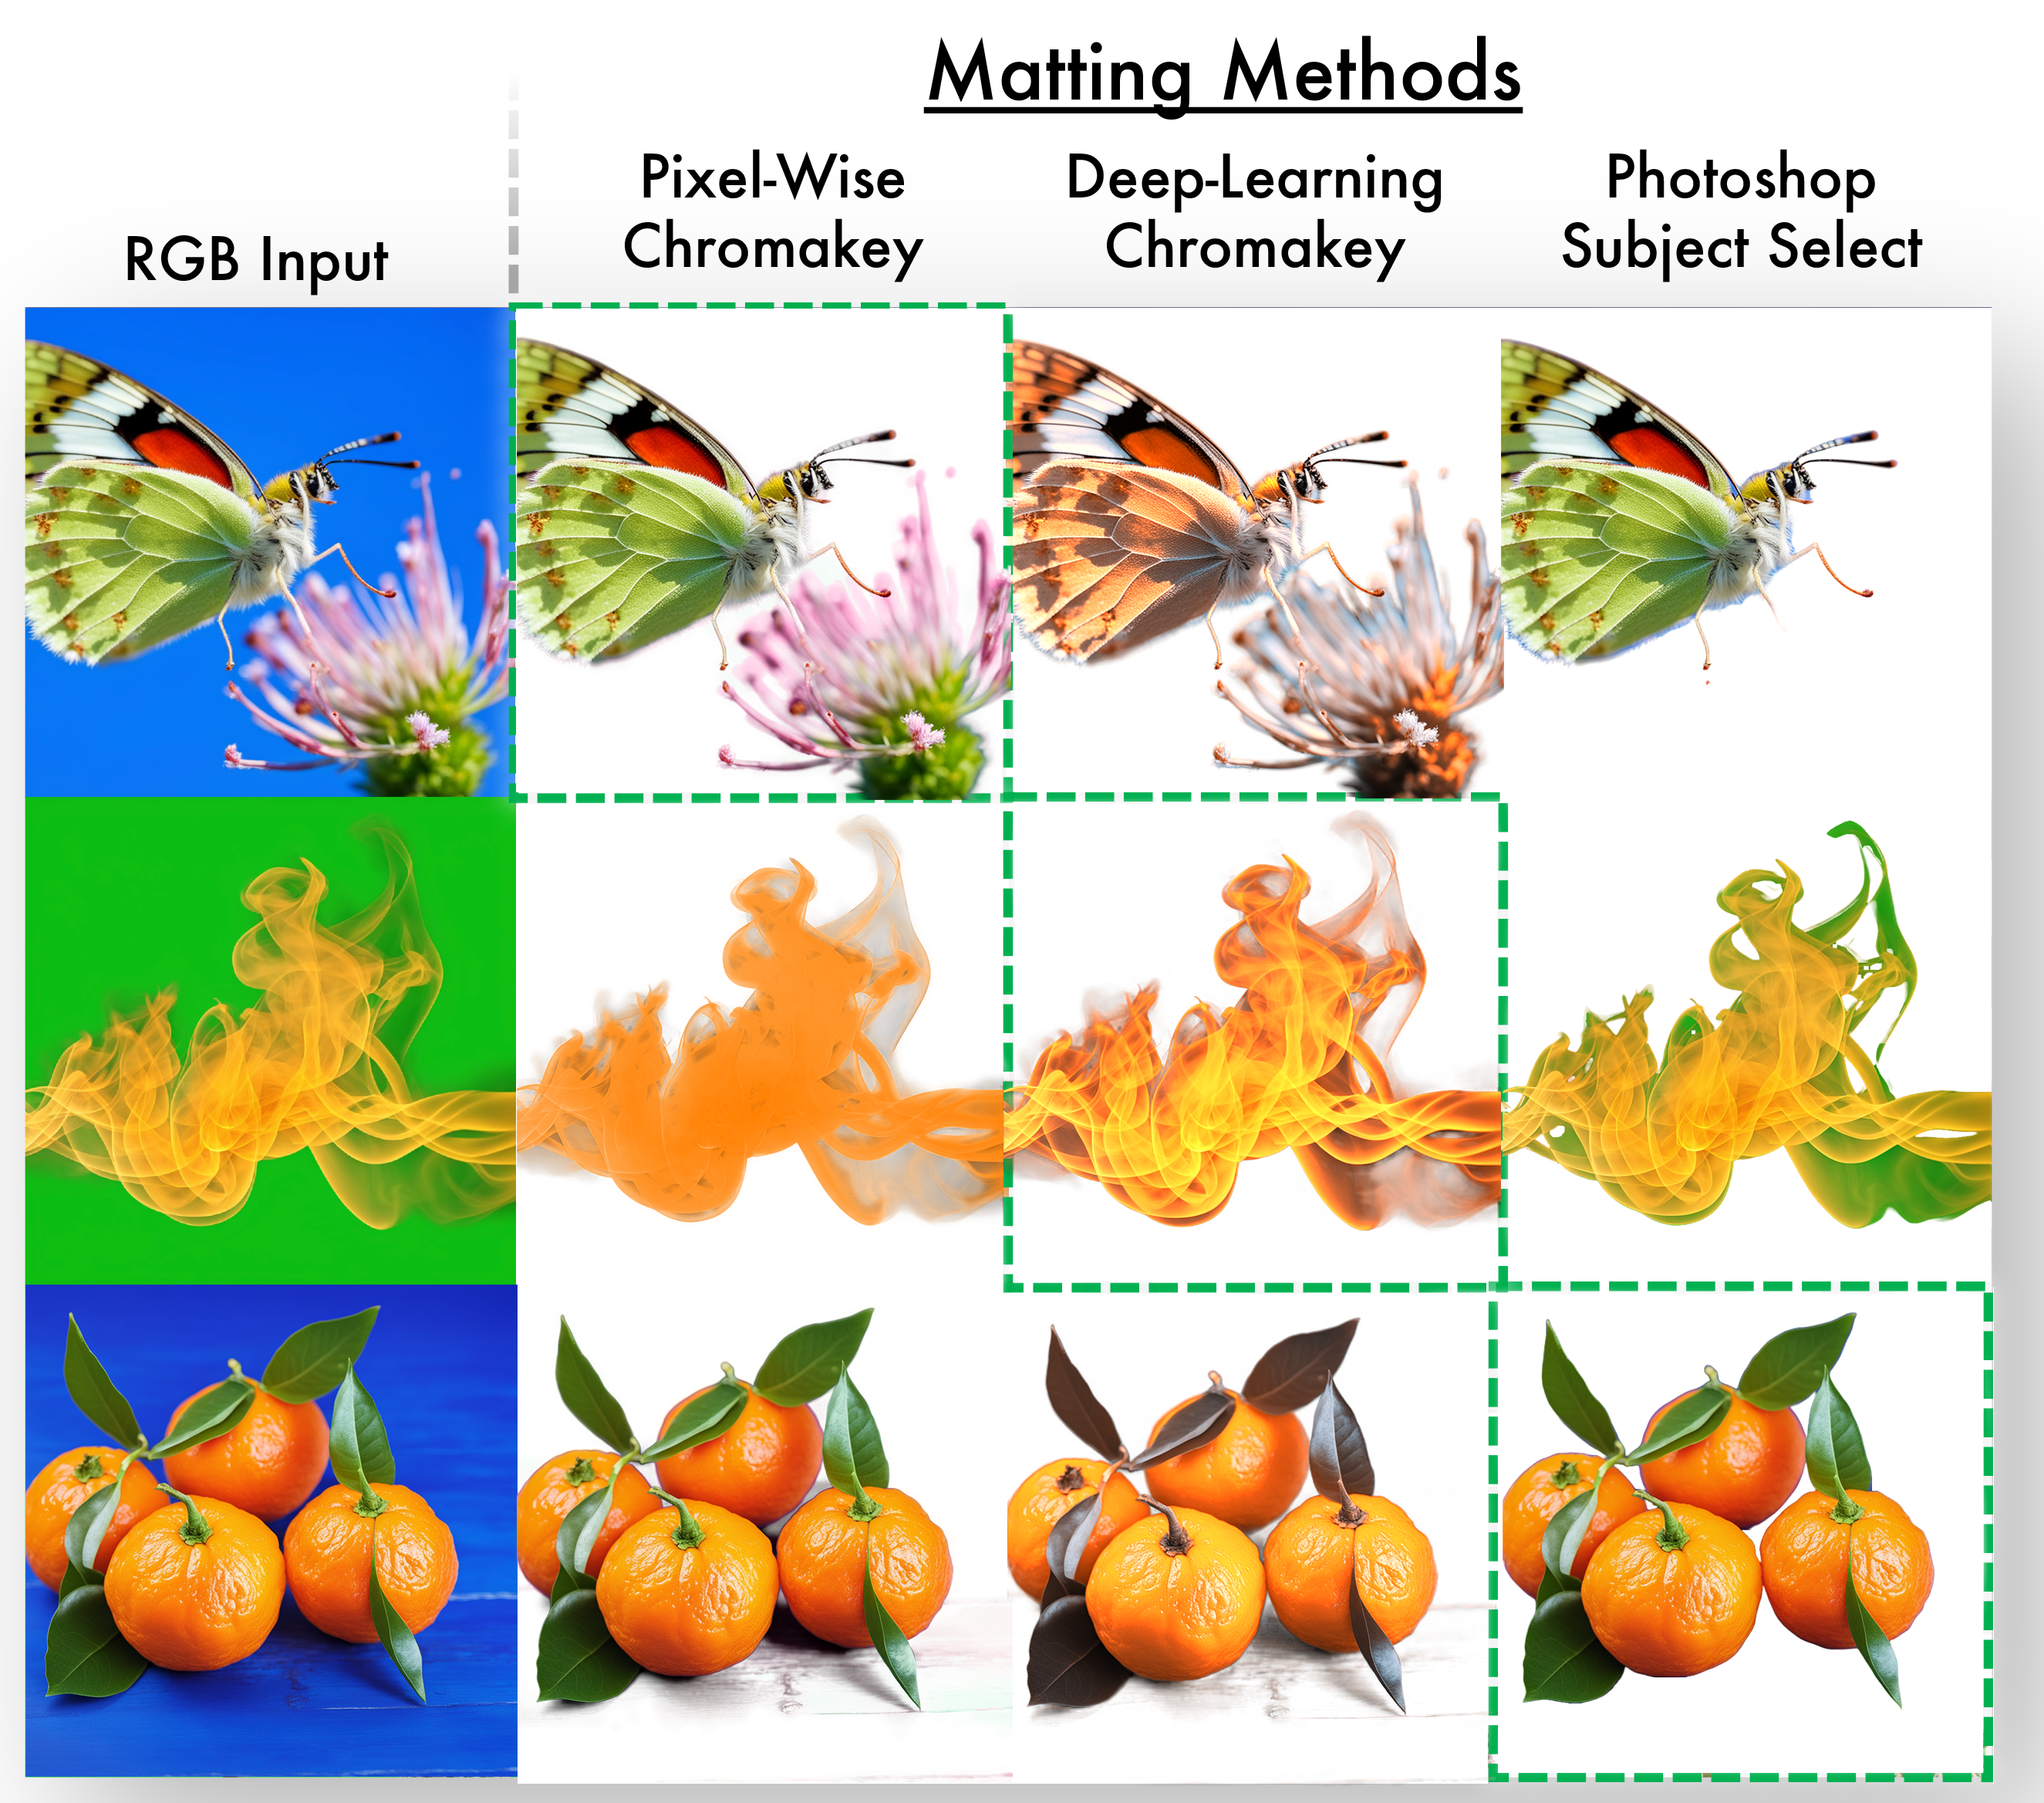
\includegraphics[width=1\linewidth]{src/3_MAGICK/figs/MattingMethods.png}
    \caption[Comparison of three matting methods]{A comparison of our three matting methods on different input images. The green dotted rectangles indicate the best result for each example.
    }
    \label{magick_fig:alpha_compare}
\end{figure}



\subsubsection{Image Selection Process}
\label{magick_sub:image_selection_process}
The last step in our dataset creation pipeline is to select the best matte. Each subject will have multiple matted results, and the goal of this step is to choose the best one. We propose a simple automatic process that can approve a large number of the images. For those failing the automatic process, we fall back to having humans select the best option.

\paragraph{Automatic Selection Process}
Each of our alpha extraction methods operate differently, with one being color-based, one being trained for computing alpha from greenscreen images, and one being designed for general object extraction. Because of this, they tend to make different mistakes. However, for cases where our method successfully produced a \emph{keyable} image, the three alpha extraction methods often produce nearly identical results. We use this as an indication that the alpha computation was successful and each of the resulting alphas are good.

To measure the similarity, we devise a similarity score metric taking into account both their alpha and RGB values - but not penalizing differences in RGB values if the alpha values are both low. To do this, we compare both RGBA images composited on different backgrounds (white and black) and take the mean similarity between these two composite images. We measure this similarity using MSSSIM~\cite{MSSSIM} (multi-scale structural image similarity) as we found it gave the best results empirically.

MSSSIM is a metric that measures similarity between images on a scale from 0 to 1, assuming the pixel values are also between 0 and 1. Given our three RGBA images $I_0$, $I_1$, and $I_2$, a white image $W$, a black image $B$, the composition function $\mathcal{C}$ and the MSSSIM function $\mathcal{M}$, we compute our similarity score $\mathcal{S}$ as:
\begin{equation}
\begin{split}
    \mathcal{S} = min_{(a,b)} \mathcal{F}(I_a, I_b) \text{\ \ \ where\ } a,b \in \{0,1,2\}  \\
    \mathcal{F}(I_a,I_b) = \frac{1}{2} (  \mathcal{M}[\mathcal{C}(I_a,W),\mathcal{C}(I_b,W)] \\
                            + \mathcal{M}[\mathcal{C}(I_a,B),\mathcal{C}(I_b,B)] )
\end{split}
\end{equation}
\cref{magick_fig:simility_comparison} shows a visual comparison between images with a high and a low similarity score.

\cref{magick_fig:similarityScoreHistogram} shows the distribution of similarity scores. Most images have very high similarity scores, indicating our process to make the images \emph{keyable} was largely successful. The median score is 0.984. We found that the top 50\% of samples (measured by similarity score) yield decent results, resulting in 110,000 images in our dataset being automatically selected. These objects tend to be solid objects including objects with hair or fur, and tend to not be objects with significant transparencies. For these automatically-selected images, we choose the pixel-wise chroma keying algorithm as it often gives the highest detail.

\paragraph{Manual Selection Process}
For images that do not fall above the threshold of automatic selection, we rely on humans to select the best alpha for us.  These tend to be subjects that contain difficult transparencies such as glass, water, smoke, or fire. We acquired 40,000 images using manual selection of the computed mattes.

We've created a program that will be released to the public along with our dataset to aid in manual selection.
It presents multiple combinations of alpha and $F$ and allows changing the background colors and zooming for accurate assessment of details, as well as additional features such as tagging images. It also serves as an efficient way to quickly view and audit the dataset. See the Appendix for details.


\begin{figure}
    \centering
    \includegraphics[width=1\linewidth]{src/3_MAGICK/figs/sim_score_qualitative2.pdf}
    \caption[Qualitative comparison of similarity scores]{A qualitative comparison of a high and low similarity score. Note how the alpha masks and colors are different between samples on the one with low similarity, but nearly identical on the one with high similarity.}
    \label{magick_fig:simility_comparison}
\end{figure}

\begin{figure}
    \centering
    \includegraphics[width=1\linewidth]{src/3_MAGICK/figs/simScoreDistribution2.pdf}
    \caption[Distribution of similarity scores in the MAGICK dataset]{The distribution of similarity scores in the dataset.}
    \label{magick_fig:similarityScoreHistogram}
\end{figure}
